\documentclass{beamer}
\usepackage{basileabeam}
\usepackage{german}
\usepackage{tikz}
\usetikzlibrary{positioning}
\usetikzlibrary{shapes,arrows}
\definecolor{baselmint}{RGB}{165,215,210}
\definecolor{baselanthrazit}{RGB}{45,55,60}
%notes
%\pgfpagesuselayout{2 on 1}[a4paper,border shrink=5mm]
%\setbeamertemplate{note page}[plain]
%\setbeameroption{show notes on second screen=bottom}

\title              {Versionsverwaltung mit Git}

\author             {Silvan Heller \textless silvan.heller@unibas.ch\textgreater\\
	\tiny{Slides für CS108: Marcel Neidinger \textless m.neidinger@unibas.ch\textgreater}}
\email              {}
\institute          {Department Mathematik \& Informatik, Universität Basel}

\date               {HS17-- Software Engineering}

\ulogo        		{Template/header}
\ulistelement    	{Template/listelement}

\graphicspath{{Images/}}
\begin{document}
\begin{frame}[t,plain]
\titlepage
\end{frame}

\begin{frame}{Recap: Programmier-Projekt?}
	\begin{itemize}
		\item Ihr seid nicht mehr alleine am Entwickeln. 
		\item Wie \textbf{synchronisiert} man die Daten?
		\item Wie vermeidet man \textbf{Datenverlust}?
		\item Wie werden \textbf{Änderungen nachverfolgt}?
	\end{itemize}
\end{frame}
\begin{frame}{Dateiserver}
	\begin{itemize}
		\item \textit{Dateiserver} oder \glqq Dropbox\grqq
	\end{itemize}
	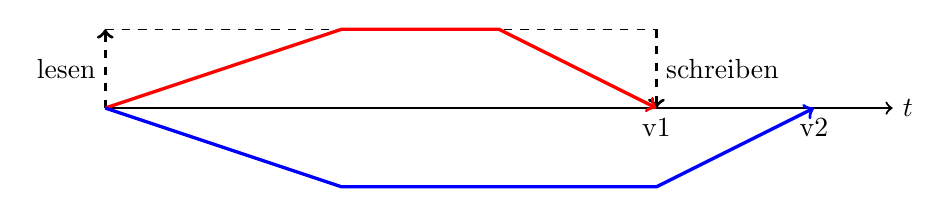
\begin{tikzpicture}
		\node[left] at (0,0.5) {lesen};
		\draw[dashed] (0,1) -- (7,1);
		\draw[->,dashed,very thick] (0,0) -- (0,1);
		\draw[->,dashed,very thick] (7,1) -- (7,0);
		\node[right] at (7,0.5) {schreiben}; 
		
		\draw[->,thick] (0,0) -- (10,0) node[right] {$t$};
		%\draw[fill=red,red] (7,0) circle(1pt);
		\draw[red,very thick,->] (0,0) -- (3,1) -- (5,1) -- (7,0) node[below,black] {v1};
		%\draw[fill=blue,blue] (9,0) circle(1pt);
		\draw[blue,very thick,->] (0,0) -- (3,-1) -- (7,-1) -- (9,0) node[below,black] {v2};
	\end{tikzpicture}
	\begin{itemize}
		\item Änderungen aus \textbf{v1} gehen verloren!
	\end{itemize}
\end{frame}
\begin{frame}{Verbesserung: Blockierender Dateiserver}
	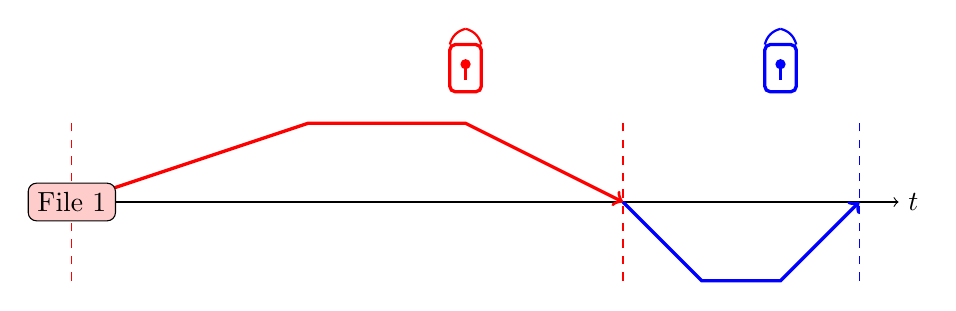
\begin{tikzpicture}
		\draw[dashed,red] (0,-1) -- (0,1);
		\draw[->] (0,0) -- (10.5,0) node[right] {$t$};
		\draw[red, very thick,->] (0,0) -- (3,1) -- (5,1) -- (7,0);
		\node[rounded corners=3pt, draw, fill=red!20] at (0,0) {File 1};
		\draw[red, rounded corners=2pt, very thick] (4.8,2) rectangle (5.2, 1.4);
		\draw[red,thick] (4.8,2) to[bend left] (5,2.2);
		\draw[red,thick] (5,2.2) to[bend left] (5.2,2);
		\draw[red,thick] (5,1.7) -- (5,1.55);
		\draw[red,thick,fill=red] (5,1.75) circle(0.05cm);
		
		% lock blue
		\draw[blue,very thick,->] (7,0) -- (8,-1) -- (9,-1) -- (10,0);
		\draw[blue, rounded corners=2pt, very thick] (8.8,2) rectangle (9.2, 1.4);
		\draw[blue,thick] (8.8,2) to[bend left] (9,2.2);
		\draw[blue,thick] (9,2.2) to[bend left] (9.2,2);
		\draw[blue,thick] (9,1.7) -- (9,1.55);
		\draw[blue,thick,fill=blue] (9,1.75) circle(0.05cm);
		
		% lock lines
		\draw[dashed,red] (7,-1) -- (7,1);
		\draw[dashed,blue] (10,-1) -- (10,1);
	\end{tikzpicture}
	\begin{itemize}
		\item \textbf{Lock-modify-unlock}
		\item Verzögerungen: gleichzeitiges Arbeiten nicht möglich
		\item Administrativer Aufwand: Was wenn vergessen wird zu entsperren?
		\item Äbhängigkeiten von Quelltextdateien werden ausser Acht gelassen 
	\end{itemize}
\end{frame}
\begin{frame}{Die Lösung}
	\begin{center}
		
\includegraphics[width=.8\linewidth]{Images/git_logo.png}
	\end{center}
\end{frame}

\begin{frame}{Git}
	\begin{center}
		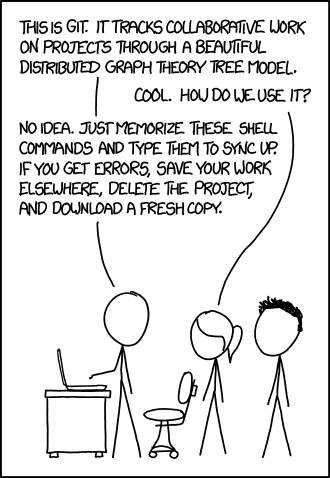
\includegraphics[width=.4\linewidth]{Images/xkcd.png}
	\end{center}
\end{frame}

\begin{frame}{Theorie: Das Baummodell}
	\begin{minipage}{0.3\textwidth}
		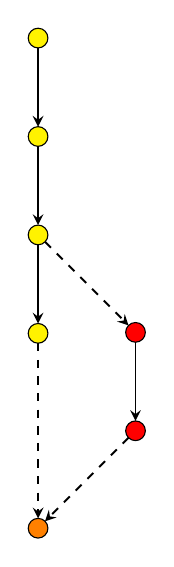
\begin{tikzpicture}[startstop/.style={circle,
                                        inner sep=0mm,outer sep=0,
                                        draw=black, 
										minimum width=0.25cm,
                                      },
					commitconnection/.style={
									line width=0.25mm,	
									->,
									>=stealth
									}
                     ]
  \node[startstop,fill=yellow] (A)  { };
  \node[startstop,below= 1cm of A,fill=yellow] (B)  { };
  \node[startstop,below= 1cm of B,fill=yellow] (C) { };
  \node[startstop,below right= 1.5cm of C,fill=red] (D) { };
  \node[startstop,below= 1cm of C, fill=yellow] (E) { };
  \node[startstop,below= 1cm of D, fill=red] (F) { };
  \node[startstop,below left= 1.5cm of F, fill=orange] (G) { };
  \draw [commitconnection]  (B) -- (C);
  \draw [commitconnection]  (A) -- (B);
  \draw [commitconnection, dashed]  (C) -- (D);
  \draw [commitconnection] (C) -- (E);
  \draw [commitconnection] (D) -- (F); 
  \draw [commitconnection,dashed] (E) -- (G);
  \draw [commitconnection,dashed] (F) -- (G);

  \end{tikzpicture}
	\end{minipage}
	\hfill\begin{minipage}{0.69\textwidth}
		\begin{description}
			\item[Commit] Status (Änderungen) eures Codes
		\end{description}
		\begin{itemize}
			\item Jeder \textbf{Commit} hat eindeutigen Hash
		\end{itemize}
		
		\begin{center}
			\includegraphics<1>[width=.9\linewidth]{Images/18333fig0303-tn.png}
			\includegraphics<2>[width=.9\linewidth]{Images/18333fig0304-tn.png}
			\includegraphics<3>[width=.9\linewidth]{Images/18333fig0307-tn.png}
						\includegraphics<4>[width=.9\linewidth]{Images/18333fig0309-tn.png}
		\end{center}
	\end{minipage}
\end{frame}
\begin{frame}{Theorie: Verteilte Versionsverwaltung}
	\begin{center}
		\begin{tikzpicture}
			\node [label={\large Origin},cloud, draw,cloud puffs=10,cloud puff arc=120,inner sep=-0.25cm,fill=blue!10] at (2,2.5) {\resizebox{0.05\linewidth}{!}{\begin{tikzpicture}[startstop/.style={circle,
                                        inner sep=0mm,outer sep=0,
                                        draw=black, 
										minimum width=0.25cm,
                                      },
					commitconnection/.style={
									line width=0.25mm,	
									->,
									>=stealth
									}
                     ]
  \node[startstop,fill=yellow] (A)  { };
  \node[startstop,below= 1cm of A,fill=yellow] (B)  { };
  \node[startstop,below= 1cm of B,fill=yellow] (C) { };
  \node[startstop,below right= 1.5cm of C,fill=red] (D) { };
  \node[startstop,below= 1cm of C, fill=yellow] (E) { };
  \node[startstop,below= 1cm of D, fill=red] (F) { };
  \node[startstop,below left= 1.5cm of F, fill=orange] (G) { };
  \draw [commitconnection]  (B) -- (C);
  \draw [commitconnection]  (A) -- (B);
  \draw [commitconnection, dashed]  (C) -- (D);
  \draw [commitconnection] (C) -- (E);
  \draw [commitconnection] (D) -- (F); 
  \draw [commitconnection,dashed] (E) -- (G);
  \draw [commitconnection,dashed] (F) -- (G);

  \end{tikzpicture}}};
			\node [label={\large Dev A},cloud, draw,cloud puffs=10,cloud puff arc=120,inner sep=-0.25cm] at (5,6) {\resizebox{0.05\linewidth}{!}{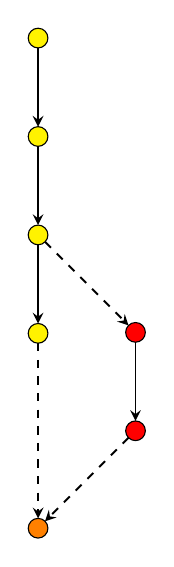
\begin{tikzpicture}[startstop/.style={circle,
                                        inner sep=0mm,outer sep=0,
                                        draw=black, 
										minimum width=0.25cm,
                                      },
					commitconnection/.style={
									line width=0.25mm,	
									->,
									>=stealth
									}
                     ]
  \node[startstop,fill=yellow] (A)  { };
  \node[startstop,below= 1cm of A,fill=yellow] (B)  { };
  \node[startstop,below= 1cm of B,fill=yellow] (C) { };
  \node[startstop,below right= 1.5cm of C,fill=red] (D) { };
  \node[startstop,below= 1cm of C, fill=yellow] (E) { };
  \node[startstop,below= 1cm of D, fill=red] (F) { };
  \node[startstop,below left= 1.5cm of F, fill=orange] (G) { };
  \draw [commitconnection]  (B) -- (C);
  \draw [commitconnection]  (A) -- (B);
  \draw [commitconnection, dashed]  (C) -- (D);
  \draw [commitconnection] (C) -- (E);
  \draw [commitconnection] (D) -- (F); 
  \draw [commitconnection,dashed] (E) -- (G);
  \draw [commitconnection,dashed] (F) -- (G);

  \end{tikzpicture}}};
			\node [label={\large Dev B},cloud, draw,cloud puffs=10,cloud puff arc=120,inner sep=-0.25cm] at (8,2) {\resizebox{0.05\linewidth}{!}{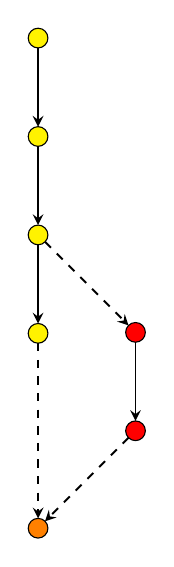
\begin{tikzpicture}[startstop/.style={circle,
                                        inner sep=0mm,outer sep=0,
                                        draw=black, 
										minimum width=0.25cm,
                                      },
					commitconnection/.style={
									line width=0.25mm,	
									->,
									>=stealth
									}
                     ]
  \node[startstop,fill=yellow] (A)  { };
  \node[startstop,below= 1cm of A,fill=yellow] (B)  { };
  \node[startstop,below= 1cm of B,fill=yellow] (C) { };
  \node[startstop,below right= 1.5cm of C,fill=red] (D) { };
  \node[startstop,below= 1cm of C, fill=yellow] (E) { };
  \node[startstop,below= 1cm of D, fill=red] (F) { };
  \node[startstop,below left= 1.5cm of F, fill=orange] (G) { };
  \draw [commitconnection]  (B) -- (C);
  \draw [commitconnection]  (A) -- (B);
  \draw [commitconnection, dashed]  (C) -- (D);
  \draw [commitconnection] (C) -- (E);
  \draw [commitconnection] (D) -- (F); 
  \draw [commitconnection,dashed] (E) -- (G);
  \draw [commitconnection,dashed] (F) -- (G);

  \end{tikzpicture}}};
		\end{tikzpicture}
	\end{center}
\end{frame}
\begin{frame}{Theorie: Branchingmodel}
	\resizebox{\linewidth}{!}{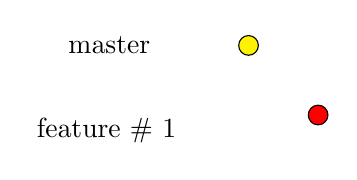
\begin{tikzpicture}[startstop/.style={circle,
                                        inner sep=0mm,outer sep=0,
                                        draw=black, 
										minimum width=0.25cm,
                                      },
					commitconnection/.style={
									line width=0.25mm,	
									->,
									>=stealth
									}
                     ]
\node[startstop,fill=yellow] (A) { };
\node[left=1cm of A,left,align=left] {master};
\node[startstop,below right=1cm of A,fill=red] (B) { };
\node[below left=1cm of A,align=left] {feature \# 1};
\end{tikzpicture}}
\end{frame}

\begin{frame}{Praxis: Konfiguration}
	\begin{block}{Konfiguration}
		\begin{itemize}
			\item \texttt{git config --global user.name ''Dein Name'' } 
			\item \texttt{git config --global user.email ''Unibas Mail''}
		\end{itemize}
		Allgemeine Konfiguration eures Userprofils, damit Github / Gitlab Eure commits zuordnen kann.
	\end{block}
\end{frame}

\begin{frame}{Terminologie: Git versus Gitlab / Github}
		\begin{itemize}
			\item \textit{git} ist eine in C geschriebene Applikation für verteilte Systemverwaltung (https://github.com/git/git)
			\item \textit{Github} und \textit{Gitlab} sind Firmen, welche Infrastruktur \& User Interfaces für git zur Verfügung stellen.
			\item \textit{SmartGit, GitKraken, SourceTree, TortoiseGit} sind alles auch UIs um die Kommandozeile zu verwenden
		\end{itemize}
\end{frame}

\begin{frame}{Praxis: Klonen und Verändern}
	\begin{block}{Klonen}
		\begin{itemize}
			\item \texttt{git clone <Repo Url> } 
		\end{itemize}
		Repository klonen \rightarrow herunterladen
	\end{block}
	\begin{block}{Verändern}
		\begin{itemize}
			\item \texttt{git add <Dateiname>}
			\item \texttt{git add .}
		\end{itemize}
		Fügt bestimmte Änderung oder alle Änderungen dem (lokalen!) Repository hinzu
	\end{block}
\end{frame}

\begin{frame}{Praxis: Commiten und Übertragen}
	\begin{block}{Commiten}
		\begin{itemize}
			\item \texttt{git commit -m ''<Nachricht>''}
		\end{itemize}
		Commitet alle änderungen (lokal!)
	\end{block}
	\begin{block}{Pushen}
		\begin{itemize}
			\item \texttt{git push origin master}
		\end{itemize}
		Pusht alle lokalen Änderungen auf \texttt{origin} in den Branch \texttt{master}
	\end{block}
\end{frame}

\begin{frame}{Git in den Übungen}
	\begin{block}{Commandline versus IntelliJ versus tool}
		\begin{itemize}
			\item IntelliJ kann alles was Ihr braucht
			\item Ihr dürft aber auch etwas anderes benützen
		\end{itemize}
	\end{block}
	\begin{block}{Fork}
		\begin{itemize}
			\item Ihr forkt das Ganttproject repo.
			\item Pro Übungsblatt ein branch
			\item Abgabe via Pull Request auf master
		\end{itemize}
	\end{block}
\end{frame}


\begin{frame}{Git: Best Practices}
	\begin{itemize}
		\item \textbf{Oft Committen} - Dem Server tut das nicht weh!
		\item Genau eine funktionale Änderung pro Commit
		\item Nur \emph{funktionierenden} Code committen
		\item Sinnvolle Commit-Kommentare schreiben. Das vereinfacht es zu verstehen was geändert wurde.
		\item Jeweils \emph{vor} dem Committen updaten
		\item 'Pull before you push' - Also nicht wie bei Türen
	\end{itemize}
	\textbf{Gut}
	
	\texttt{Fehler \#32 behoben - GUI stürzt ohne Port Paramter nicht mehr mit Null-Pointer Exception ab}\\[1.5em]
	\textbf{Schlecht} 
	
	\texttt{Zeugs gemacht - Dinge geändert}
\end{frame}

\begin{frame}{Git: Cheatsheet}
	\begin{itemize}
		\item Textuelle Zusammenfassung: \url{http://gitref.org/basic/}
		\item Traditionelles Cheatsheet: \url{https://www.git-tower.com/blog/git-cheat-sheet/}
	\end{itemize}
\end{frame}
\begin{frame}[t,plain]
\lastpage{{\usebeamerfont{title} Fragen?}}
\end{frame}

\end{document}

